\section{Thermal Data and Oscilloscope Captures}
\label{app:thermal}
On the bench the hottest die rose from 25--28\,$^\circ$C at 200\,kHz to 29--31\,$^\circ$C at 300 and 400\,kHz (\cref{fig:thermal}), consistent with the dead-time commutation loss behind $R_{sw}$, which grows as $\fsw^3$, while the open-loop residual and the current-loop gain fall; 300\,kHz balanced the two. The highest reading on either day was 39\,$^\circ$C, in full sun at 200\,kHz, far below the 85\,$^\circ$C trip.

\begin{figure}[htbp]
  \centering
  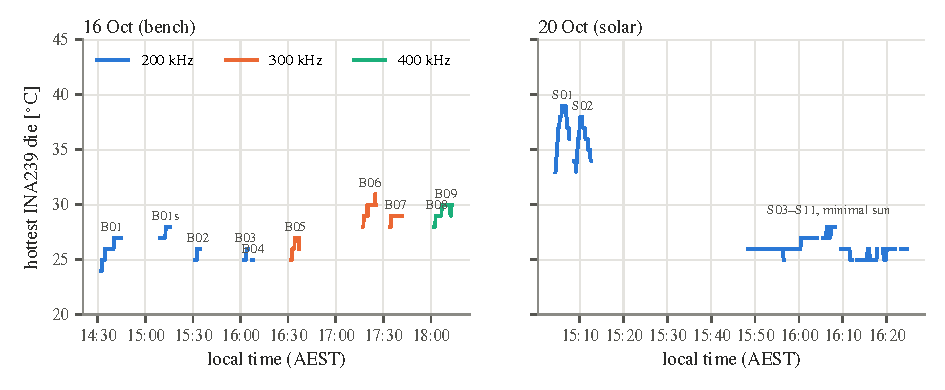
\includegraphics[width=\linewidth]{results/thermal}
  \caption[{Hottest INA239 die temperature in every test window}]{Hottest INA239 die temperature during every test window (10\,s maxima of the telemetry), coloured by switching frequency. The over-temperature trip is at 85\,$^\circ$C (INA die) and 80\,$^\circ$C (heatsink, Pi-side E-stop).}
  \label{fig:thermal}
\end{figure}
\begin{figure}[htbp]
  \centering
  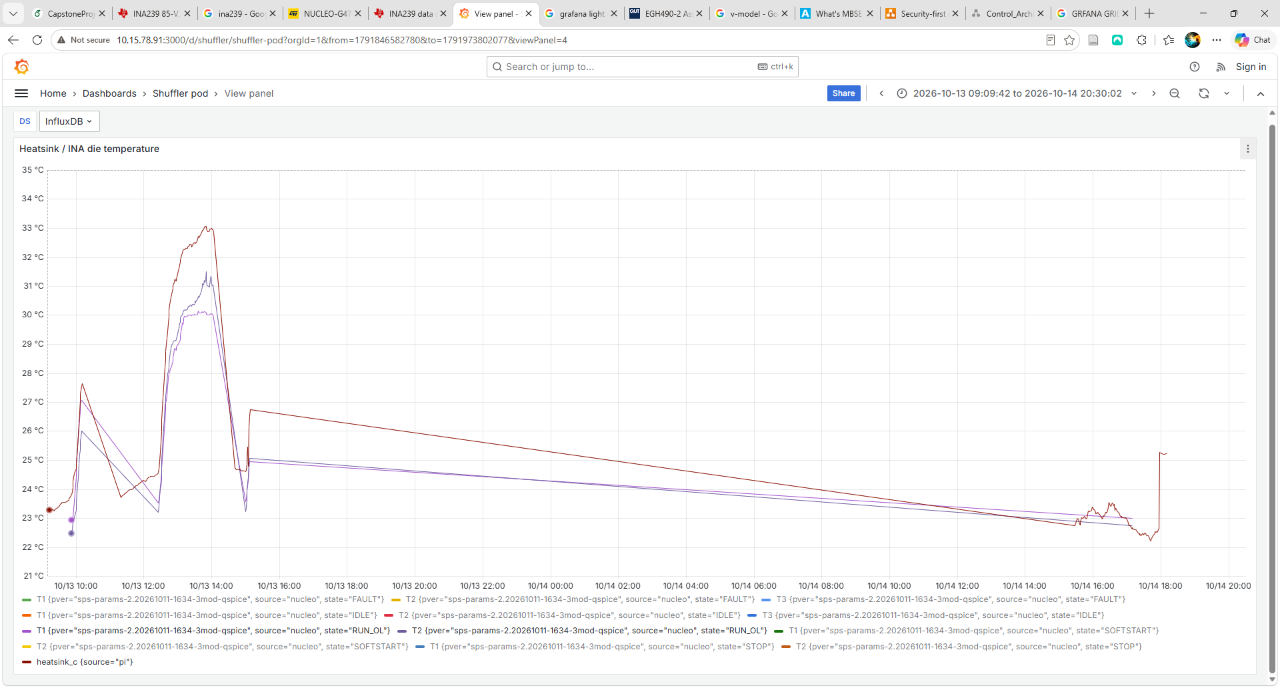
\includegraphics[width=0.7\linewidth]{misc/thermal_100k}
  \caption{Grafana capture of the 100\,kHz open-loop exploration on 13--14 Oct, which ran but behaved erratically.}
\end{figure}
\begin{figure}[htbp]
  \centering
  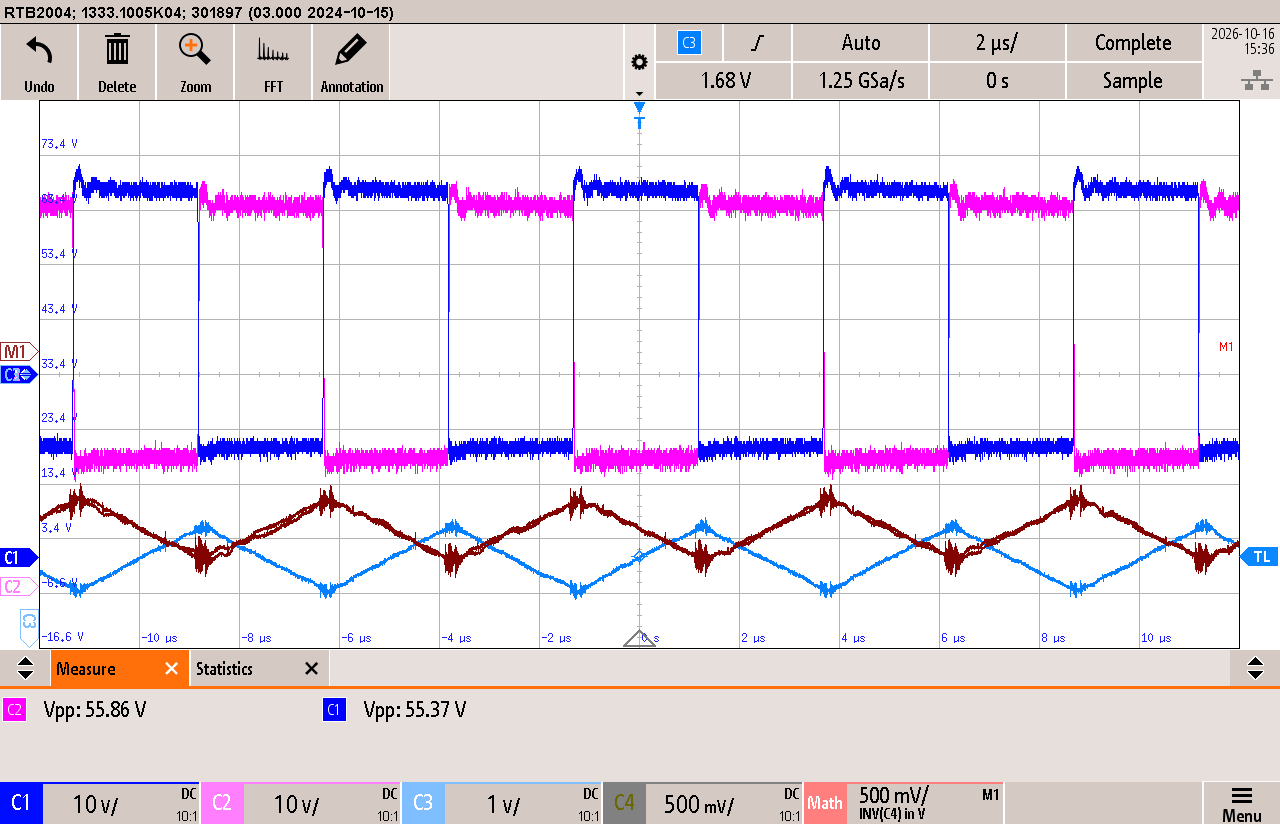
\includegraphics[width=0.32\linewidth]{misc/scope_200k}\hfill
  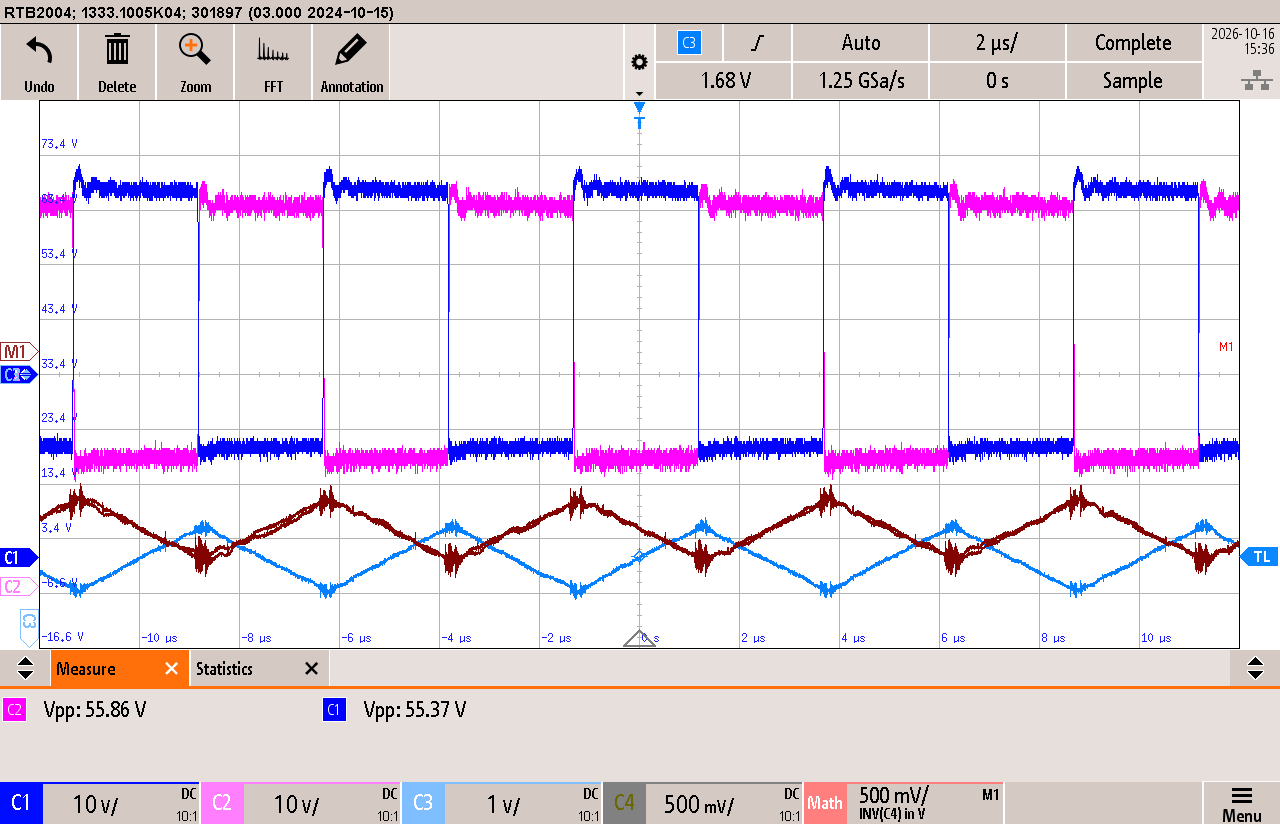
\includegraphics[width=0.32\linewidth]{misc/scope_300k}\hfill
  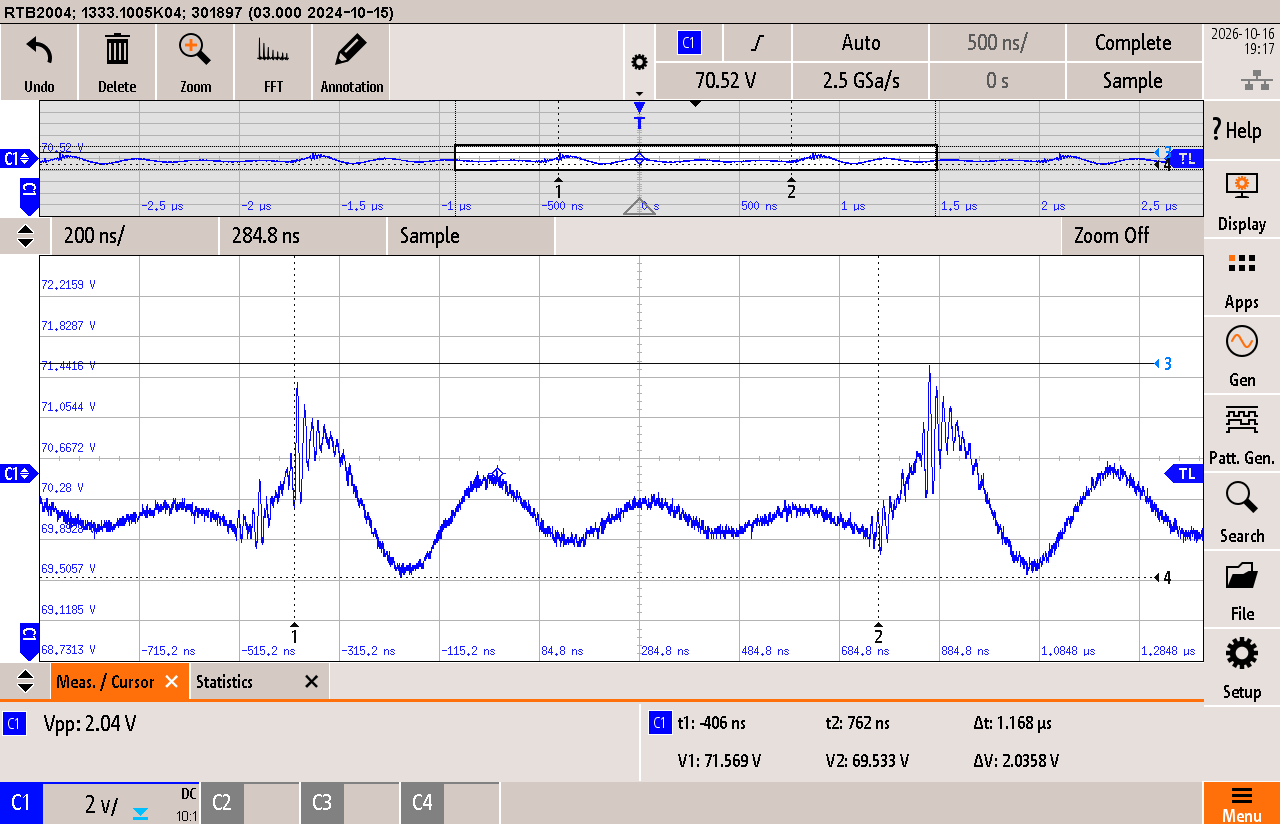
\includegraphics[width=0.32\linewidth]{misc/scope_400k}
  \caption{Oscilloscope captures of the switch-node waveforms at 200, 300 and 400\,kHz (dead time and 180$^\circ$ interleave check).}
  \label{fig:scope}
\end{figure}
